% This LaTeX was auto-generated from MATLAB code.
% To make changes, update the MATLAB code and export to LaTeX again.

\documentclass{article}

\usepackage[utf8]{inputenc}
\usepackage[T1]{fontenc}
\usepackage{lmodern}
\usepackage{graphicx}
\usepackage{color}
\usepackage{hyperref}
\usepackage{amsmath}
\usepackage{amsfonts}
\usepackage{epstopdf}
\usepackage[table]{xcolor}
\usepackage{matlab}

\sloppy
\epstopdfsetup{outdir=./}
\graphicspath{ {./ConstantVelocityLinear2D_KF_images/} }

\begin{document}

\begin{par}
\begin{flushleft}
Specify the initial state estimate to have zero velocity.
\end{flushleft}
\end{par}

\begin{matlabcode}
x = 0.2;
y = 0.3;
initialState = [x;0;y;0];
KF = trackingKF('MotionModel','2D Constant Velocity','State',initialState);
\end{matlabcode}


\begin{matlabcode}
disp(KF.StateTransitionModel);
\end{matlabcode}
\begin{matlaboutput}
     1     1     0     0
     0     1     0     0
     0     0     1     1
     0     0     0     1
\end{matlaboutput}
\begin{matlabcode}
disp(KF.MeasurementModel);
\end{matlabcode}
\begin{matlaboutput}
     1     0     0     0
     0     0     1     0
\end{matlaboutput}


\begin{par}
\begin{flushleft}
Create the measured positions from a constant-velocity trajectory.
\end{flushleft}
\end{par}

\begin{matlabcode}
vx = 0.2;
vy = 0.1;
T  = 0.5;
pos = [0:vx*T:2;0:vy*T:1]';
pos = pos + 0.05*randn(size(pos));
\end{matlabcode}


\begin{par}
\begin{flushleft}
Predict and correct the state of the object.
\end{flushleft}
\end{par}

\begin{matlabcode}
for k = 1:size(pos,1)
    pstates(k,:) = predict(KF,T);
    cstates(k,:) = correct(KF,pos(k,:));
end
\end{matlabcode}


\begin{par}
\begin{flushleft}
Plot the tracks.
\end{flushleft}
\end{par}

\begin{matlabcode}
plot(pos(:,1),pos(:,2),'k.', pstates(:,1),pstates(:,3),'+', ...
    cstates(:,1),cstates(:,3),'o')
xlabel('x [m]')
ylabel('y [m]')
grid
xt  = [x-2 pos(1,1)+0.1 pos(end,1)+0.1];
yt = [y pos(1,2) pos(end,2)];
text(xt,yt,{'First measurement','First position','Last position'})
legend('Object position', 'Predicted position', 'Corrected position')
\end{matlabcode}
\begin{center}
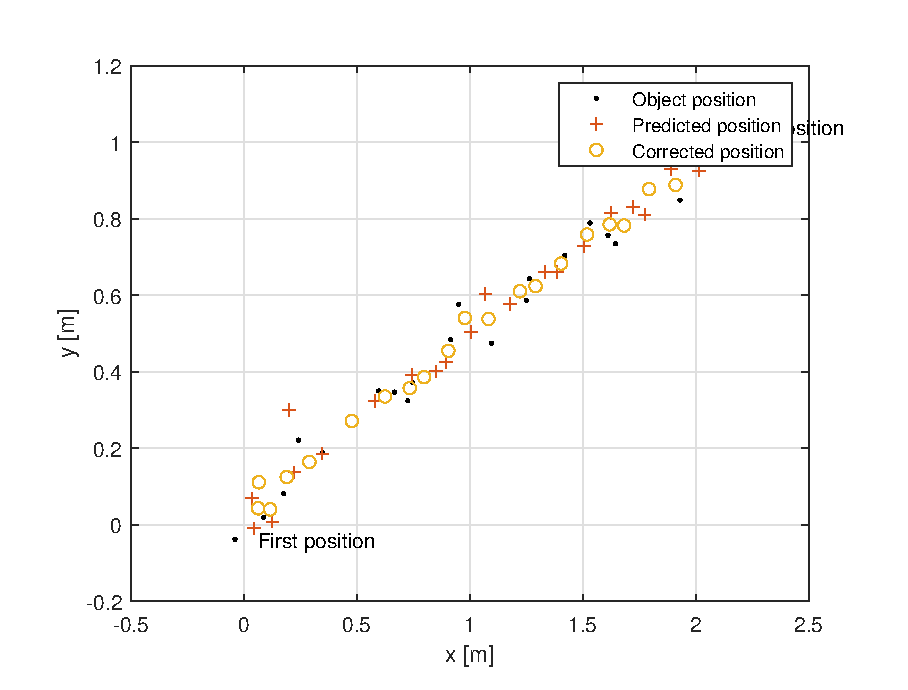
\includegraphics[width=\maxwidth{56.196688409433015em}]{figure_0.eps}
\end{center}

\end{document}
